% !TeX spellcheck = en_GB
\section{Introduction to Bayesian statistics}

\subsection{Bayesian basics}

The Bayesian approach is based on the idea, that a prior distribution of the data is assumed and the model is adjusted to this prior.

To perform a Bayesian Data Analyses the following things are required:
\begin{description}
	\tightlist
	\item[observed Data] The data you want to have conclusions from
	\item[generativer Model] to generate new data according to your prior
	\item[prior information] quantify the uncertainty of parameters in your model (i.e. by including prior information)
\end{description}

\subsubsection{Workflow for Binomial models}
\begin{enumerate}
	\tightlist
	\item Run $n$ simulations of possible $\theta$ using the prior distribution.
	\begin{lstlisting}
prior = runif(n)
	\end{lstlisting}
	\item Build a generative model, which simulates the model based on the prior distribution of $\theta$.
	\begin{lstlisting}
generativemodel = function(theta) {
	rbinom(1, nSamples, theta)
}
	\end{lstlisting}
	\item Simulate $n$ times using the generative model
	\begin{lstlisting}
simdata = rep(NA, n)
for(i in 1:n) {
	simdata[i] = generativemodel( prior[i] )
}
	\end{lstlisting}
	\item Calculate the posterior by checking which simulation resulted in the measured value(s)
	\begin{lstlisting}
posterior = prior[simdata == nSignedUp]
	\end{lstlisting}
\end{enumerate}

Step 2 and 3 can be made in one step, in case the generative model is as simple as in the shown example:
\begin{lstlisting}
simdata = rbinom(n, nSamples, prior)
\end{lstlisting}

\paragraph{Inference}
If a posterior is given, the following code snippets can be used for inference:
\begin{lstlisting}
mean(posterior) # the mean success rate
quantile(posterior, c(0.05, 0.95)) # the 90% confidence interval

# What's the probability of a success rate higher than x
sum(posterior[posterior>x])/length(posterior)

# If the experiment is repeated m samples, how big is the success rate
successForM <- rbinom(length(posterior), m, posterior)
\end{lstlisting}

\subsubsection{Possible prior distributions}

\paragraph{Uniform}
In case there is no knowledge about the distribution of $\theta$ the uniform distribution should be used. For the prior the uniform distribution must have its limits at 0 and 1.

\paragraph{Beta distribution}
\begin{gather*}
X\sim Beta(a, b)\\
E(X) = \frac{a}{a+b}\\
Var(X) = \frac{ab}{(a+b+1)(a+b^2)}\\
mode(X) = \frac{a-1}{a+b-2}
\end{gather*}

Mode = position of $f(x)_{max}$.

\begin{figure}[H]
	\centering
	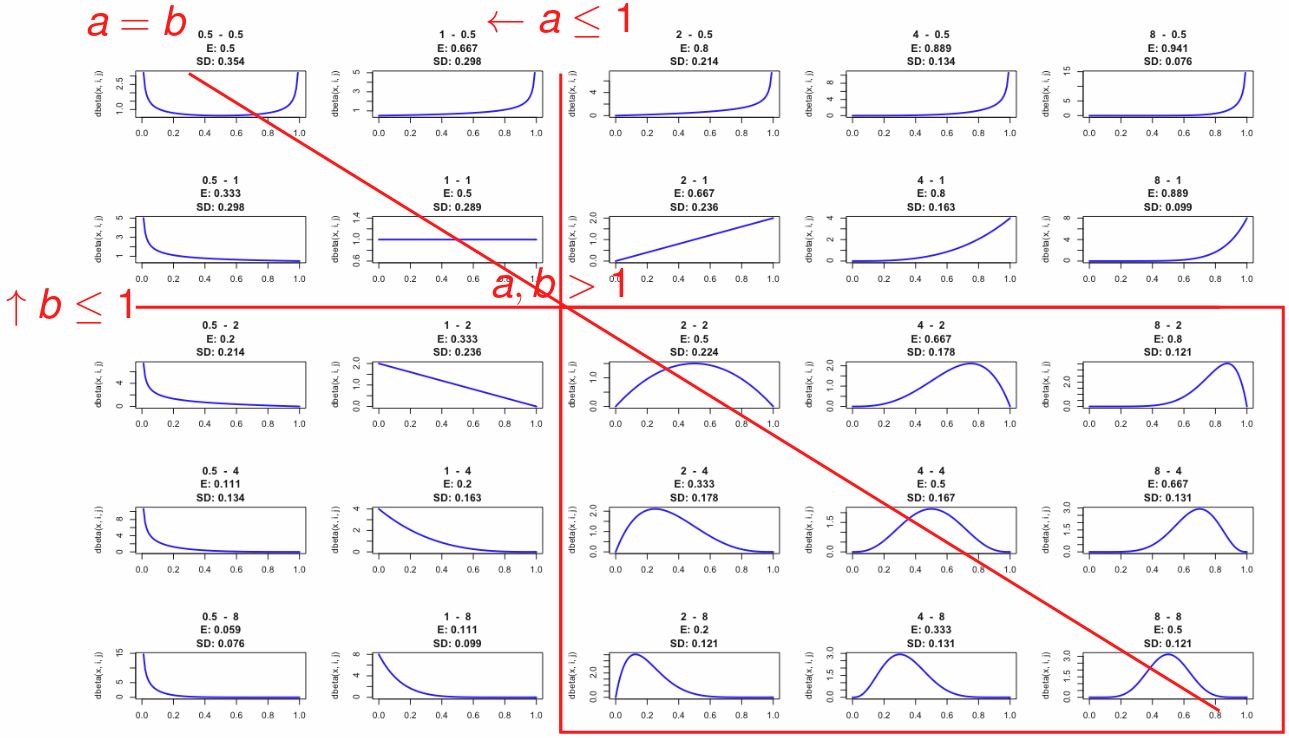
\includegraphics[width=\textwidth]{images/beta-examples.png}
	\caption{Examples of the beta distribution using different a and b values}
\end{figure}

\paragraph{Gamma distribution}
\begin{gather*}
X\sim Gamma(a, b)\\
E(X) = \frac{a}{b}\\
Var(X) = \frac{a}{b^2}\\
mode(X) = \frac{a-1}{b} (if \; a \geq 1)
\end{gather*}

\paragraph{Beta-binomial}
The Beta-binomial distribution is a Binomial distribution with N trials in which the probabilities of success are randomly drawn from a Beta(a, b) distribution.
\begin{gather*}
X\sim BetaBinom(N, a, b)\\
E(X) = N\frac{a}{a+b}\\
Var(X) = N\frac{ab}{(a+b)^2}\frac{a+b+N}{a+b+1}
\end{gather*}

\paragraph{Comparison with the frequentist approach}
Bayesian is an extension of the frequnetist approach. If not sure, start with a flat prior, the result is identical.

\subsection{Approximate Bayesian computation}
\subsubsection{Conditional probability}
\begin{gather*}
P(A|B) = \frac{P(A\cap B)}{P(B)}\\
P(A,B) = P(A|B)P(B) + P(B|A)P(A)\\
\Rightarrow P(A|B) = \frac{P(B|A)P(A)}{P(B)} = \frac{P(B|A)P(A)}{\sum_{i=1}^{n}P(B|A_i)P(A_i)}
\end{gather*}

For Bayesian modeling:
\begin{equation*}
P(\theta|D) = \frac{P(D|\theta)P(\theta)}{P(D)} = \frac{P(D|\theta)P(\theta)}{\sum_{i=1}^{n}P(D|\theta_i)P(\theta_i)} \propto P(D|\theta)P(\theta)
\end{equation*}

\subsubsection{Rejection algorithm}
Instead of throwing away all samples where the simulated data is not equal to the real data, one can set a small threshold $\epsilon$ to collect $||D_i-D||<\epsilon$ with $D$ as the Data and $D_i$ as simulated data. 

\subsection{A/B testing}
A/B testing is a way to compare two alternatives, typically by testing a subjects' response to variant A against variant B, and determining which of the two variant is more effective.

\mbox{}\\
This can be achieved by ``fitting'' two models and test the confidence intervals of parameter $\theta_A$ and $\theta_B$.

\begin{lstlisting}
A.prior = runif(n)
B.prior = runif(n)

A.sim = rbinom(n, numSamples, A.prior)
B.sim = rbinom(n, numSamples, B.prior)

ind = ((A.sim == A.success) & (B.sim == B.success))
A.posterior = A.prior[ind]
B.posterior = B.prior[ind]
\end{lstlisting}

\paragraph{Profit maximization}
Is a special case of A/B testing where one of the variants might be more effective but more expensive, too. In this case, the profit maximization can be calculated using $\theta$ and the expected gain.
\begin{equation*}
profit_i = \theta \cdot (income_i - cost_i)
\end{equation*}

\subsection{Discrete probability models}
Until now, we simulated and conditioned on observed data, to get a random sample from the posterior. A more analytical approach is to use a special prior distribution, which is called the \textbf{conjugate prior}.

\mbox{}\\
\textbf{Conjugate prior}: A prior distribution for a given generative model (a.k.a. likelihood function) which results in the same family for the posterior distribution.

\subsubsection{Binomial model}
The conjugate prior for the binomial model is the beta distribution.

\begin{equation*}
	L(\theta) = P(D|\theta) = {{n}\choose{s}}\theta^s(1-\theta)^{n-s}
\end{equation*}

With $L(\theta)$ as Likelihood, $n$ the number of trials and $s$ the number of success.

If the prior is beta distributed, the posterior will be beta distributed, too:
\begin{gather*}
\theta\sim Beta(a, b)\\
\theta|D\sim Beta(a+s, b+n-s)
\end{gather*}

=> The more samples, the lower the influence of the initial $a$ and $b$.

\subsubsection{Geometric distribution}
The geometric distribution takes values in $\mathbb{N}_0$. It represents the number of failures in a sequence of Bernoulli trials before a success occurs.
\begin{gather*}
P(X=n|\theta) = \theta(1-\theta)^n\\
E(X) = \frac{1-\theta}{\theta}\\
Var(X) = \frac{1-\theta}{\theta^2}
\end{gather*}

With a $Beta(a,b)$ distributed prior, the posterior distribution is:
\begin{gather*}
\theta|D\sim Beta(a+1, b+x) = Beta(a+1, b+\sum_{i=1}^{n}x_i)
\end{gather*}
With $x_i$ being the number of failures in experiment i before a success occurred.

\subsubsection{Poisson model}
This model counts the number of rare events in a fixed interval of time or space if these occur randomly and independent of each other with a constant rate.
\begin{gather*}
X\sim Pois(\lambda)\\
E(X) = \lambda\\
Var(X) = \lambda
\end{gather*}

The conjugate prior for the Poisson model is the Gamma distribution.
\begin{gather*}
\lambda \sim Gamma(a, b)\\
\lambda|D \sim Gamma(a+\sum_{i=1}^{n}x_i, b+n)
\end{gather*}
With $x_i$ being the number of events within the $i$th period and $n$ the number of periods.

\subsubsection{Hypergeometric distribution}
Basically the binomial distribution without replacement. It represents the number of $m$ success in $n$ draws without replacement from a set of size $N$ containing exactly $M$ objects with a certain feature.
\begin{gather*}
X\sim HyperGeo(n,N,M)\\
P(X=m|n, N, M) = \frac{{{M}\choose{m}}{{N-M}\choose{n-m}}}{{N\choose n}}\\
E(X) = n\frac{M}{N}\\
Var(X) = n\frac{M}{N}\frac{N-M}{N}\frac{N-n}{N-1}
\end{gather*}

With a Beta-binomial prior on M i.e. $M\sim BetaBin(N, a, b)$ the posterior distribution of M is:
\begin{equation*}
M-m\sim BetaBin(N-n, a+m, b+n-m)
\end{equation*}

\subsubsection{Exponential model}
The exponential distribution takes values in $\mathbb{R}_0^+$ representing the waiting time until the occurrence of an event.
\begin{gather*}
X\sim Exp(\lambda)\\
p(x) = p(x|\lambda) = \lambda e^{-\lambda x}\\
E(X) = {1\over\lambda}\\
Var(X) = {1\over\lambda^2}
\end{gather*}

The conjugate prior for the exponential model is the Gamma distribution. With $\lambda\sim Gamme(a, b)$ as prior, the posterior is:
\begin{equation*}
\lambda|D\sim Gamma(a+n, b+\sum_{i=1}^{n}t_i)
\end{equation*}

\paragraph{Properties}
The exponential distribution is \textbf{memoryless}. The waiting time until a certain event occurs, does not depend on how much time has elapsed already. The probability for the time to the next event stays the same and is independent when you start the observation.

\mbox{}\\
Consider you have n identical components. Each component has the same failure rate $\lambda$. Then, the failure rate for observing a failure in one of the $n$ components is $n\lambda$.

\subsubsection{Gaussian distribution}
The Gaussian or Normal distribution is very common in statistics and takes values in $\mathbb{R}$. The central limit theorem shows that under weak conditions i.i.d. observations converge to a normal distribution.
\begin{gather*}
X\sim Norm(\mu, \sigma^2)\\
E(X) = Mode(X) = \mu\\
Var(X) = \sigma^2
\end{gather*}

\begin{figure}[H]
	\centering
	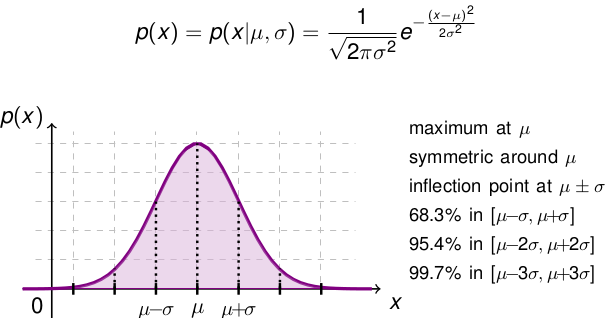
\includegraphics[width=.7\textwidth]{images/gaussian-details.png}
	\caption{Some details of the Gaussian distribution}
\end{figure}

\paragraph{Conjugate prior for $\mu$}
Our data has a distribution of $X\sim Norm(\mu, \sigma^2)$ with a fixed standard deviation $\sigma$. With a normal prior $\mu\sim Norm(m, s^2)$ the posterior distribution for $\mu$ is:
\begin{equation*}
\mu|D\sim Norm\left((\frac{m}{s^2}+\frac{\sum_{i=1}^{n}x_i}{\sigma^2})(\frac{1}{s^2}+\frac{n}{\sigma^2})^{-1}, (\frac{1}{s^2}+\frac{n}{\sigma^2})^{-1}\right)
\end{equation*}

\paragraph{Conjugate prior for $\sigma$}
Our data has a distribution of $X\sim Norm(\mu, \sigma^2)$ with a fixed mean $\mu$. With a Gamma(a, b) prior on the precision $\tau$, where $\tau = \frac{1}{\sigma^2}$ the posterior distribution of $\tau$ is:
\begin{equation*}
\tau|D\sim Gamma\left(a+\frac{n}{2}, b+\frac{\sum_{i=1}^{n}(x_i-\mu)^2}{2}\right)
\end{equation*}

\subsection{Markov chain Monte Carlo (MCMC) methods}

\subsubsection{Monte carlo method}

The idea of Monte Carlo simulation is to use i.i.d. samples of a random generator with density $p$ to approximate expectations.

\paragraph{Stochastic integration}
One possible usage of the Monte Carlo simulation is to integrate a complex function stochastically:
\begin{lstlisting}
# f: function to integrate
f = function(x){return(x^2*cos(.6*x)+.2)}
n = 1000
hits = 0

# simulate in area -1, 2 for X and 0, 2 for Y
# -> dX = 3, dY = 2
x_ = runif(n, -1, 2)
y_ = runif(n, 0, 2)

hits = sum(y_<f(x_))

area = hits/n * (3*2) # dX * dY
\end{lstlisting}

\subsubsection{Markov chain}
\begin{figure}[H]
	\centering
	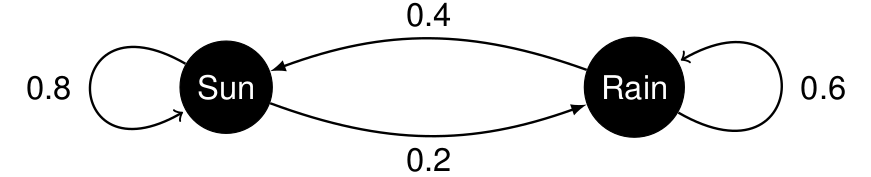
\includegraphics[width=0.6\textwidth]{images/markov-chain-example.png}
	\caption{Example of a Markov Chain}
\end{figure}

\paragraph{Equilibrium/stationary distribution}
Every \textbf{ergodic} (irreducible and aperiodic) Markov chain has a stationary distribution $\pi$.\\
Definitions:
\begin{description}
	\tightlist
	\item[irreducible] A Markov Chain is irreducible if it is possible to get from any state to any other state.
	\item[periodic] A Markov chain is periodic if you can visit certain states only at periodically recurrent time steps. Otherwise, a Markov chain is called \textbf{aperiodic}.
\end{description}

The stationary distribution can be found by the following equation:
\begin{gather*}
\pi_x = \sum_{y\in S}\pi_y\cdot P_{y\rightarrow x}\\
\sum_{i=1}^{n}\pi_i = 1
\end{gather*}

\paragraph{Detailed balance}
A Markov chain has the property of ``detailed balance'' in case it ends in the stationary distribution $\pi$ independent of the state, the chain started in. If $\pi$ fulfils the following equation, \textbf{detailed balance} is given:
\begin{equation*}
\pi_x\cdot P_{x\rightarrow y} = \pi_y\cdot P_{y\rightarrow x}
\end{equation*}

\subsubsection{Metropolis hastings}
A metropolis hastting has the following components:
\begin{description}
	\tightlist
	\item[A data generating distribution $Q$] To sample new proposals, a data generation distribution $Q$ is required.
	\item[A prior distribution] The prior distribution of the parameter (can be uniform)
	\item[A posterior distribution] with a prior distribution of each parameter(s)
\end{description}

Idea:
\begin{enumerate}
	\tightlist
	\item Proposal: Simulate $z\sim Q$ and set $\theta_{prop} = \theta + z$
	\item Metropolis Rejection: Simulate $u\sim Unif(0, 1)$\\
	If $\frac{\pi(\theta_{prop})Q(\theta|\theta_{prop})}{\pi(\theta)Q(\theta_{prop}|\theta)}>u$ set $\theta = \theta_{prop}$
\end{enumerate}
Remarks: In case $\theta_{prop}$ is better than $\theta$,  $\theta_{prop}$ will always be updated (fraction gets positive). $u$ is a random parameter describing a ``how much worse parameter'' is accepted. In case the probability density function of $Q$ is symmetric (e.g. uniform or normal distribution), $Q(\theta|\theta_{prop}) = Q(\theta_{prop}|\theta)$. Therefore, the metropolis rejection is simplified:\\
If $\frac{\pi(\theta_{prop})}{\pi(\theta)}>u$ set $\theta = \theta_{prop}$
\begin{lstlisting}
nrSignups =  6
nrTotal   = 16

nSimulations = 100000

signUpRate_i = runif(1)

sample_signUpRates = rep(NA,nSimulations)
for(i in 1:nSimulations)
{
	# data generation Q
	signUpRate_prop = runif(1)
	u = runif(1)
	if( u < (dbinom(nrSignups,nrTotal,signUpRate_prop)/dbinom(nrSignups,nrTotal,signUpRate_i)))
	{
		signUpRate_i = signUpRate_prop
	}
	sample_signUpRates[i] = signUpRate_i
}

# throw away burn in samples
signUpRates = sample_signUpRates[500:nSimulations]
\end{lstlisting}

With $beta(4, 20)$ prior:
\begin{lstlisting}
nrSignups =  6
nrTotal   = 16

nSimulations = 100000

signUpRate_i = runif(1)

sample_signUpRates = rep(NA,nSimulations)
for(i in 1:nSimulations)
{
	# data generation Q
	signUpRate_prop = runif(1)
	u = runif(1)
	# the prior is only included here
	if( u < (dbinom(nrSignups,nrTotal,signUpRate_prop)*dbeta(4, 20)/dbinom(nrSignups,nrTotal,signUpRate_i))*dbeta(4, 20))
	{
		signUpRate_i = signUpRate_prop
	}
	sample_signUpRates[i] = signUpRate_i
}

# throw away burn in samples
signUpRates = sample_signUpRates[500:nSimulations]
\end{lstlisting}

\subsubsection{Full probabilistic model}
Metropolis hasting with multiple parameters.
\begin{figure}[H]
	\centering
	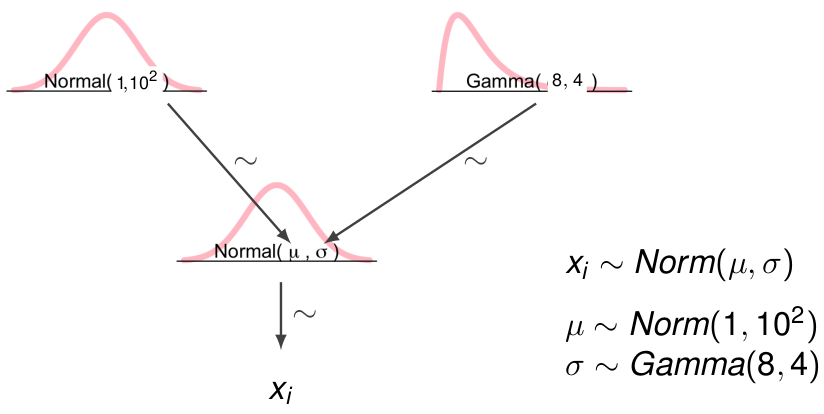
\includegraphics[width=0.6\textwidth]{images/full-probalistic-example.png}
	\caption{Example of a full probabilistic model.}
\end{figure}

\begin{lstlisting}
obs = c(2.27, 1.17, 3.58, 3.95, 3.13, -1.50, 4.71, 2.58, 4.05, 5.20)
m = rnorm(1,1,10)
s = rgamma(1,8,4)
m_sample = s_sample = c()
# Bayesian Data Analysis via MCMC
for(i in 1:10000) {
	mean_prop = rnorm(1,m,0.1)
	sd_prop = abs(rnorm(1,s,0.1))
	# R = product of P(x|D), P(mu|D), P(sigma|D) for each observation
	R = prod(dnorm(obs,mean_prop,sd_prop))*dnorm(mean_prop,1,10)* dgamma(sd_prop,8,4)/prod(dnorm(obs,m,s))/dnorm(m,1,10)/dgamma(s,8,4)
	u = runif(1,0,1)
	if( R > u ) {
		m = mean_prop
		s = sd_prop
	}
	m_sample = c(m_sample,m)
	s_sample = c(s_sample,s)
}
\end{lstlisting}

Often $R$ is calculated by using the logarithmic posterior, to simplify calculation.
\begin{lstlisting}
# Observed data:
obs_x = runif(12,0,10)
obs_y = 3 * obs_x + 2 + rnorm(12,mean=0,sd=1)

# Log of (unnormalized) posterior density
logPosterior = function(b0_, b1_, sigma_){
	sum(dnorm(b0_+b1_*obs_x - obs_y, 0, sigma_, log=T))
}
# Starting value
b0 = runif(1,0,1)
b1 = runif(1,0,1)
sigma = runif(1,0,1)
# Collect sample
b0_sample = c()
b1_sample = c()
sigma_sample = c()
for(i in 1:10000) {
	b0_prop = rnorm(1,b0,0.1) # Q~Norm(0, 0.1)
	b1_prop = rnorm(1,b1,0.1)
	s_prop = abs(rnorm(1,sigma,0.1))
	R = exp(logPosterior(b0_prop, b1_prop, s_prop)-logPosterior(b0, b1,
	sigma))
	u = runif(1,0,1)
	if( u < R) {
		b0 = b0_prop
		b1 = b1_prop
		sigma = s_prop
	}
	b0_sample = c(b0_sample,b0)
	b1_sample = c(b1_sample,b1)
	sigma_sample = c(sigma_sample,sigma)
}
\end{lstlisting}

\subsubsection{Chain with filters}
\begin{figure}[H]
	\centering
	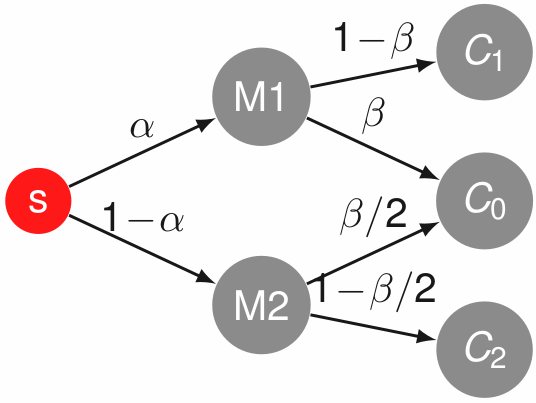
\includegraphics[width=0.3\textwidth]{images/filter-chain.png}
	\caption{An example filter chain}
\end{figure}

Find ``Posterior'' with $c_0=400, $$c_1=1200$ and $c_2=900$:\\
\begin{equation*}
(\alpha\cdot (1-\beta))^{1200}\cdot((1-\alpha)(1-\beta/2))^{900}\cdot (\alpha\cdot\beta + (1-\alpha)\beta/2)^{400}
\end{equation*}
And ``logPosterior'':
\begin{equation*}
1200\cdot log(\alpha\cdot (1-\beta))+900\cdot log((1-\alpha)(1-\beta/2)) +  400\cdot log(\alpha\cdot\beta + (1-\alpha)\beta/2)
\end{equation*}
\begin{lstlisting}
# Here with additional prior distributions for a and b
logStatDist = function(a_,b_)
{
	return(1200*log(a_*(1-b_)) + 900*log((1-a_)*(1-b_/2)) + 400*log(a_*b_+(1-a_)*b_/2) + dunif(a_,0.5,1,log=TRUE) + dbeta(b_,1.1,9.9,log=TRUE))
}
# number of samples
n = 100000
# Starting value
a = runif(1,0.5,1)
b = rbeta(1,1.1,9.9)
# Collect sample
a_sample = rep(NA,n)
b_sample = rep(NA,n)
#  Bayesian Data Analysis via MCMC
for(i in 1:n)
{
	a_prop = runif(1,a-0.01,a+0.01)
	b_prop = runif(1,b-0.01,b+0.01)
	R =  exp(logStatDist(a_prop,b_prop)-logStatDist(a,b))
	u = runif(1,0,1)
	if( R > u)
	{
		a = a_prop
		b = b_prop
	}
	a_sample[i] = a
	b_sample[i] = b
}
\end{lstlisting}
